
The GVMT defines an abstract stack-based machine (The GVMT Abstract Machine) that has well defined semantics, but is abstract in the sense that it cannot execute any programs. It is designed to both assist in implementing stack-based virtual machine and allow translation to efficient machine-code.

NOTE: the term `bytecode' is used below to refer to a virtual-machine instruction and the term `instruction' is used to refer to an abstract-machine instruction. Bytecodes (virtual-machine instructions) are defined as a sequence of instructions (abstract-machine instructions).

\section{Components}
The GVMT Abstract Machine consists of main (shared) memory and zero or more threads of execution.

Each thread consists of four stacks, a transfer register, and a list of thread-local variables. The stacks are:
\begin{enumerate}
\item Data stack
\item Control stack
\item State stack
\item Native parameter stack
\end{enumerate}

The main memory is divided into two parts: a user-managed region and a garbage-collected heap.

Upon initialisation, the GVMT Abstract Machine has zero threads; no code is executing.
Threads can be added and started by using the \verb|gvmt_start_thread| function.

\section{Threads}
Each thread is independent, the number of concurrently executing threads is limited by the underlying operating sytem and hardware. Threads share the heap, but have their own stacks and thread-local variables. GVMT threads are implemented as operating sytem threads.

\subsection{Execution Model}

Execution of a thread starts by creating a new set of stacks for that thread. Initially all stacks are empty. The arguments passed to the  \verb|gvmt_start_thread| function are pushed to the data stack, followed by the address of the start function. The \verb|CALL_X| is then executed, where \verb|X| depends on the type specified in the \verb|gvmt_start_thread| function.

Execution of a function procedes as follows:
A frame containing all the temporary variables necessary for the function is pushed to the control stack. This frame becomes current frame for accessing all temporary variables. The layout and management of this frame is not defined. Temporary variables in previously pushed stacks cannot be accessed.
The first instruction in the function is then executed, proceeding to the next instruction and so on. The exception to this are flow control instruction such as \verb|HOP| or \verb|BRANCH| which may jump to a designated successor instruction. 

\subsection{Functions}

A function in GVMT is defined as a linear sequence of instructions. Execution of a function starts by pushing a frame to the control stack. This frame will have  sufficent space to store all the temporary variables required by the function. 
Execution then starts with the first instruction in the sequence and proceeds to the next instruction and so on. The exception to this are flow control instruction such as \verb|HOP| or \verb|BRANCH| which may jump to a designated successor instruction.

\subsection{Interpreters}

The interpreter acts externally like a normal function; it can be called like any other. It behaviour is substantially different from that of normal functions.
The interpreter commences execution, like a normal function, by pushing a frame to the control stack. This frame will have  sufficent space to store all the temporary variables of the bytecodes of the interpreter plus any interpreter-scope variables. The interpreter definition specifies the names and types of these variables.

Each activation of an interpreter contains a virtual-machine-level instruction pointer which tells it which bytecode to execute.
The start-point of the  interpreter is passed in as a parameter and popped from the data-stack on entry.

Execution of bytecodes (bytecodes) proceeds in a linear fashion, unless a \verb|JUMP| or \verb|FAR_JUMP| abstract-machine instruction is encountered.

The execution of individual bytecodes proceeds as follows: The abstract-machine instructions that make up that bytecode are executed in the same way as for a normal function. Should the end of the bytecode be reached (as it will be for most bytecodes) then the instruction pointer is updated to point at the next instruction and that instruction is then executed.

\subsection{Compiled Code}

The output of the compiler is a function and can be called like any other. Its behaviour, in GVMT abstract-machine 
terms\footnote{Its real-world behaviour may differ; it should be faster, and it may implement the top of the data-stack differently.}, 
is exactly the same as if the interpreter were called with the same input (bytecodes) as passed to the compiler when it generated the compiled function, provided the bytecodes are not modified.

\subsection{Abstract Machine Instructions}

GVMT abstract machine instructions. can be grouped into three categories:
\begin{description}
\item[Data] Instructions that take values on the data stack and place results there, such as addition.
\item[Flow control] Instructions that alter the flow of control, both between instructions and between bytecodes.
\item[Stack manipulation] Instructions that explicitly manipulate or describe the status of the data, control and state stacks.
\end{description}

Appendix \ref{app:inst} contains the full abstract machine instruction set.

\section{The Stacks}

\subsection{The Data Stack}

The data stack is where all arithmetic operations takes place. The instruction set is designed so that the data stack can be treated as an in-memory array, yet allow back-ends some freedom to store the top few items in registers.  See the \verb|STACK| instruction for more details on accessing the stack as an array. The data stack grows downward. The stack supports six distinct types: \verb|I4|, \verb|I8|, \verb|F4|, \verb|F8|,  \verb|p|, \verb|R|. The \verb|U4| and \verb|U8| types are also supported, but these are synonymous with the \verb|I4| and \verb|I8| types. Barring \verb|I4|/\verb|U4| and \verb|I8|/\verb|U8| pairs, pushing one type to the stack and then popping a different type is an error.

\subsection{GC Safe points}
The GC safe instruction declares that the executing thread can be interupted for garbage collection. In order for this to be safe, the following restrictions must be observed:
\begin{enumerate}
\item No non-reference values are on the data stack.
\item All heap objects reachable from this thread are in a scannable state.\footnote{Usually this means that the header(class) of any newly created object will have been initialised.}
\end{enumerate}
The front-end tools \gvmtc{} and \gvmtic{} automatically ensure that condition 1 is true for all C code.
The toolkit ensures that all virtual stack items are reachable by the garbage-collector.
Condition 2 can be ensured simply by initialising all objects immediately after allocation.

\subsection{The Control Stack}

The control stack is an opaque structure used to handle procedure calls and returns, and storing of temporary variables. Interpreter frames are also allocated on the control stack. Memory can be allocated on the call-stack, but subsequent allocation are not guaranteed to be contiguous.
The control stack will usually map directly onto the native C stack.

Temporary variables are accessed by the \verb|TLOAD_X(n)| and \verb|TSTORE_X(n)| instructions. Temporaries have no address.
Temporary variables have the same types as data stack elements, with the same restrictions on mixing types.


%         \begin{center}
%         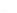
\includegraphics[scale = 0.8]{Stack.eps}
% Diagram1.eps: 300dpi, width=3.29cm, height=4.97cm, bb=0 0 388 587
%         \end{center}

\subsection{The Native Parameter Stack}
Parameters are also passed to native code using the native parameter stack. Values are pushed to the native parameter stack by the \verb|NARG_X| instructions and poppedn by the \verb|N_CALL| instruction. All functions and bytecodes must have pop exactly as many values as they push to the native value stack.

\subsection{The State Stack}
Each state object consists of the current underlying machine state (in order to resume execution from the same point), the current data-stack depth, the current control stack depth, and the current interpreter instruction pointer (if in the interpreter).

The state stack depth does not need to be recorded as it must be unchanged.

\subsection{Raise and Transfer}
The  \verb|RAISE| and \verb|TRANSFER| instructions are primarily designed to implement exception handling, but can be used to implement coroutines and continuations.

\subsection{Thread-local variables}
Each thread has thread-locals variables, the number and type of these variables are determined by the developer.

\section{The heap}
The GVMT Abstract Machine heap is a garbage collected heap. The toolkit user needs to provide a function \verb|gvmt_shape| which supplies the garbage collector with information for scanning of objects. See section \ref{sect:user-shape}.
Static roots of the heap can either be defined when the VM is built or added at runtime, see section\ref{sect:user-roots}.

\subsection{Shape\label{sect:shape}}
During tracing the garbage collector needs to know both the extent of an object and which fields are references to other objects, and which are not. The developer communicates this information to the toolkit via a `shape' vector (array).
This shape is a zero-terminated vector of integers. Each integers represents either N successive references or N successive words of non-references. References are represented by positive numbers, non-references by negative numbers (zero is the terminator).
For example the shape [ 2, -2, 1, 0 ] represents an object of total extent 5 words, the first 2 and last of which are references.
The following C declaration (taken from the example Scheme VM):
\begin{verbatim}
GVMT_OBJECT(cons) {   
    struct type *type;   // Opaque (non-GC) pointer
    GVMT_Object car;     // Reference to heap object
    GVMT_Object cdr;     // Reference to heap object
};
\end{verbatim}
defines \verb|cons| objects. These \verb|cons| objects would have a shape of [ -1, 2, 0 ].

\subsection{Garbage collection}
No garbage collection algorithm is specified for the GVMT. However, since the GVMT can support both read and write barriers as well as the declaration of GC safe points, a wide range of collectors should be feasible.
Currently both generational and non-generational collectors are available, although only `stop-the-world' collectors have been implemented. The GVMT garbage collectors also support tagging, which allows non-references to be stored in reference slots by setting one or more `tag' bits.
Read and write barriers are implemented via the \verb|RLOAD_R| and \verb|RSTORE_R| instructions respectively. 

\subsection{Exception handling}

The GVMT exception handling model uses an explicit stack, rather than tables. These means that using exceptions has a runtime cost even when the exceptions are not used as a means of flow control transfer, but that exception handling itself is much faster than for table-based approaches. The GVMT exception handling mechanism is similar to the C setjump-longjump mechanism.

The four instructions involved are (See section \ref{sect:user-except} for the matching intrinsics):
\begin{itemize}
\item [PUSH\_CURRENT\_STATE] Pushes the current execution state onto the state stack. This state-object holds the following information: The current execution point(immediately after the \verb|PUSH_CURRENT_STATE| instruction), the stack depth, and the current control stack frame. Finally it pushes NULL onto the data stack. 
\item [POP\_STATE] Pops and discards the state-object from the state stack.
\item [RAISE] Pops the value from the TOS and stores it. The state-object on top of the state stack is examined and the thread execution state (data and control stack pointers) restored to the values held in the handler. The stored value is pushed onto the data stack. Finally, execution resumes from the location stored in the state-object.
\item [TRANSFER] Pops the value from the TOS and stores it. The state-object on top of the state stack is examined and the thread execution state, except the data-stack (control stack pointer only) restored to the value held in the handler. The stored value is pushed onto the data stack. Finally, execution resumes from the location stored in the state-object.
\end{itemize}
It is an error (resulting in a probable crash) to leave a state object on the state stack after the function in which it was pushed has returned.
There is no concept of handling only some sorts of exceptions in the GVMT. All exceptions are caught; exceptions that should be handled elsewhere must be explicitly reraised. 

Exceptions work as expected in interpreted (and compiled) code, as the interpreter instruction pointer is stored along with the machine instruction pointer.

\section{Concurrency\label{sect:conc}}

The GVMT is concurrency friendly, all generated code and library code is thread-safe. The GVMT does not provide a thread library, so the developer will have to use the underlying operating system library.
Concurrency is at the thread level, the GVMT is unaware of processes.

In order that the toolkit can operate correctly, it must be informed of the creation and destruction of threads.
The toolkit provides functions for this purpose, see Section \ref{sect:user-threads} for more details.
The developer should also be aware that heap allocation may block, waiting for a collection, so locks should not be held across an allocation.

The GVMT also provides fast locks for synchronisation in the case where contention is expected to be rare. This functionality is provided by the  LOCK and UNLOCK abstract machine instructions. 

The intrinsic functions \verb|gvmt_lock(gvmt_lock_t *lock)| and \verb|gvmt_unlock(gvmt_lock_t *lock)| are translated to the LOCK and UNLOCK instructions, respectively.

\emph{Warning:} GVMT locks are not automatically unlocked by the RAISE instruction. The developer must ensure that either a RAISE cannot occur between a LOCK and UNLOCK, or that the LOCK UNLOCK pair are PROTECTed. A safe LOCK/UNLOCK sequence is:
\begin{verbatim}
gvmt_lock_t lock = GVMT_LOCK_INITIALIZER;
GVMT_Object ex;
gvmt_lock(&lock)
GVMT_BEGIN_TRY(ex)
\end{verbatim}
\nopagebreak[4]
        \vdots
\nopagebreak[4]
\begin{verbatim}
gvmt_unlock(&lock)
GVMT_CATCH
gvmt_unlock(&lock)
gvmt_raise(ex)
GVMT_END_TRY
\end{verbatim}

\subsection{Memory model}
As all threads share the same heap, they may access heap objects concurrently. The following guarantees are made about the state of the heap and roots seen from one thread when modified by another thread:

All writes to pointers(P), references(R) and integers(I) not larger than a pointer are atomic. 


The order in which changes to memory appear to one thread are the same as for another. Ie, thread 1 writes to A, then writes to B. Thread 2 will not see a change in B before it sees a change in A.


In between synchronisation points, the delay between a write being made by one thread and a write being seen by another thread is indefinite.

\section{GVMT Stack Code}
GVMT Stack Code (GSC) is the instruction set of the GVMT Abstract Machine.
GSC should be viewed as a sort of abstract assembly language. It is possible to define a virtual machine entirely in C, as the front-end tools, \gvmtic{} and \gvmtc, compile C into GSC.
It is useful, however to have some awareness of GVMT Stack Code when using the GVMT.
To get a better idea of how GSC is used, have a look at the output of \gvmtc and \gvmtic in the \verb|/example| directory.

Appendix \ref{app:inst} contains a full list of GSC instructions.
